\documentclass{article}

\usepackage{amsmath}
\usepackage{graphicx}

\addtolength{\oddsidemargin}{-.3in}
\addtolength{\evensidemargin}{-.3in}
\addtolength{\textwidth}{0.6in}

\begin{document}

\title{Homework 6\\
       OpenMP}
\author{Geoffrey Ulman\\
        CSI702}
\date{April 2010}
\maketitle

\section{Design}
Because generation of the Mandelbrot set is a truly embarrissingly parallel problem, using OpenMP to parallelize the serial code was very simple. At the core of the serial code are two nested loops which iterate through the columns and rows of the discretized Mandelbrot set grid. Because calculating a single row (the inner loop) is a relative fast operation and there are many more rows (typically 512 or 1024 in the experiments performed) than the number of available processors (typically 2 to 8 in the experiments performed), parallelizing the outer loop and performing the inner loop iterations in serial was enough to keep all available processors busy in most cases.

\section{Challenges}


\section{OpenMP Commands}
The standard \verb!#pragma omp parallel for! directive was used in front of the outer for loop in the Mandelbrot calculation. The shared and private variables were specified using \verb!default(shared)! and \verb!private(i,j,x,y,zr,zi,it,zr2,zi2)!. To facilitate performing multiple test runs without recompiling, \verb!schedule(runtime)! was used and scheduling was set using the \verb!OMP_SCHEDULE! environment variable. The number of threads used was set using the \verb!OMP_NUM_THREADS! enviroment variable.

\section{Performance Analysis}

\begin{figure}
\centering
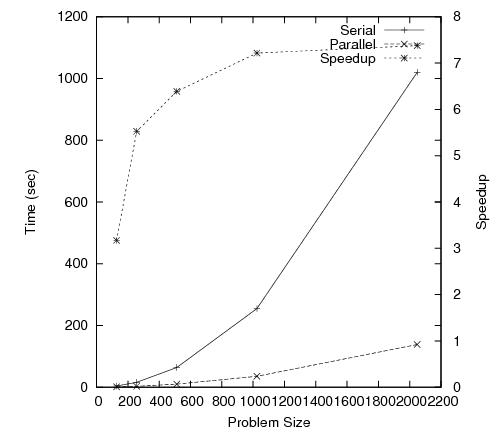
\includegraphics[width=0.7\textwidth]{../data/amazon_n.png}
\caption{Parallel and Serial Timing Results on Amazon EC2 Node with 8 Threads and Static,10 Scheduling and Variable Problem Size}
\label{amazon_n}
\end{figure}

\begin{figure}
\centering
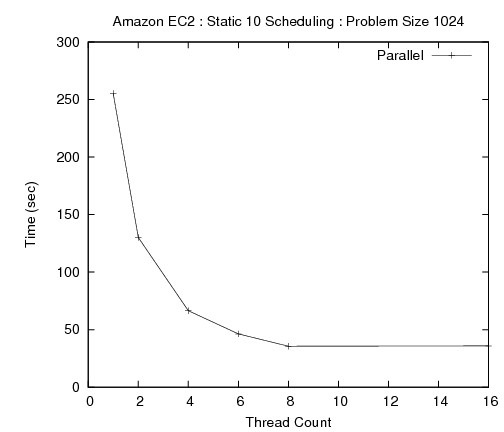
\includegraphics[width=0.7\textwidth]{../data/amazon_threads.png}
\caption{Parallel Timing Results on Amazon EC2 Node with 1024 Problem Size and Static,10 Scheduling and Variable Thread Count}
\label{amazon_threads}
\end{figure}

\begin{figure}
\centering
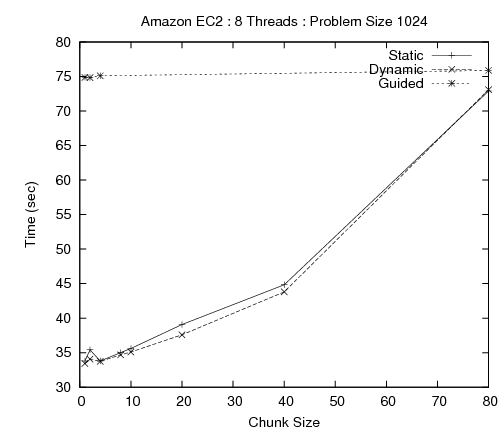
\includegraphics[width=0.7\textwidth]{../data/amazon_chunk.png}
\caption{Parallel Timing Results on Amazon EC2 Node with 1024 Problem Size and 8 Threads and Variable Scheduling}
\label{amazon_chunk}
\end{figure}







\begin{figure}
\centering
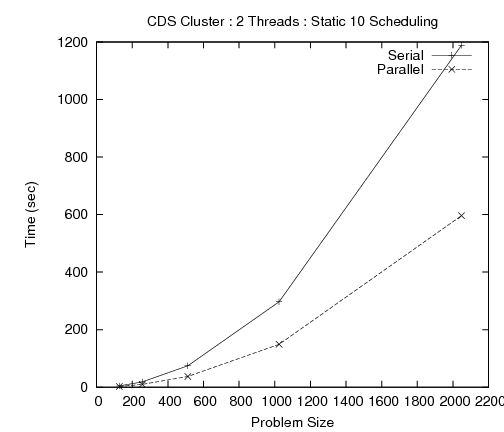
\includegraphics[width=0.7\textwidth]{../data/cds_n.png}
\caption{Parallel and Serial Timing Results on CDS Node with 8 Threads and Static,10 Scheduling and Variable Problem Size}
\label{cds_n}
\end{figure}

\begin{figure}
\centering
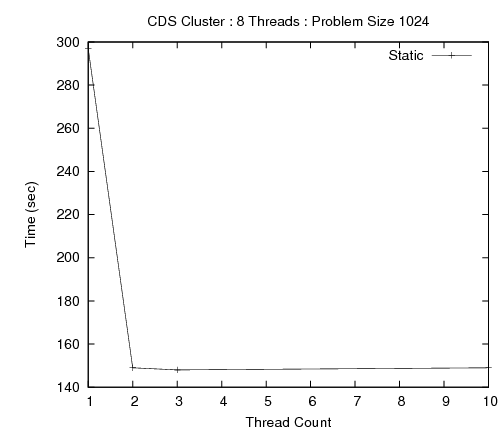
\includegraphics[width=0.7\textwidth]{../data/cds_threads.png}
\caption{Parallel Timing Results on CDS Node with 1024 Problem Size and Static,10 Scheduling and Variable Thread Count}
\label{cds_threads}
\end{figure}

\begin{figure}
\centering
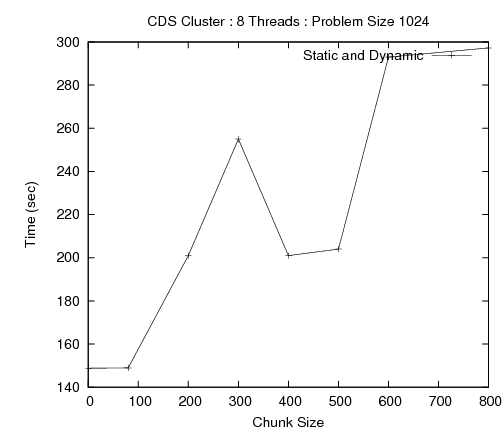
\includegraphics[width=0.7\textwidth]{../data/cds_block.png}
\caption{Parallel Timing Results on Amazon EC2 Node with 1024 Problem Size and 8 Threads and Variable Scheduling}
\label{cds_chunk}
\end{figure}




\section{Output Comparison}
\label{outputcomp}

\begin{thebibliography}{9}

\bibitem{cpl}
  Brian W. Kernighan and Dennis M. Ritchie,
  \emph{The C Programming Language},
  Prentice Hall PTR, New Jersey,
  2009.

\end{thebibliography}

\end{document}
